\subsection{Amplifying Joy: Understanding Antenna Efficiency!}

\begin{tcolorbox}[colback=gray!10, colframe=black, title=E9A09] What is antenna efficiency?
\begin{enumerate}[label=\Alph*.]
    \item Radiation resistance divided by transmission resistance
    \item \textbf{Radiation resistance divided by total resistance}
    \item Total resistance divided by radiation resistance
    \item Effective radiated power divided by transmitter output
\end{enumerate} \end{tcolorbox}

\subsubsection{Concepts Related to Antenna Efficiency}

Antenna efficiency is a critical parameter in understanding how well an antenna converts input power into radiated energy. In essence, antenna efficiency (\(\eta\)) can be defined mathematically as:

\[
\eta = \frac{R_r}{R_t}
\]

where:
- \(R_r\) is the radiation resistance of the antenna,
- \(R_t\) is the total resistance of the antenna.

\subsubsection*{Understanding Radiation Resistance:}

Radiation resistance is a measure of how effectively an antenna can radiate electromagnetic energy as a function of the input power. It is a component of the total resistance seen by the feed point of the antenna and is typically determined by the antenna design and its radiation pattern.

\subsubsection*{Total Resistance:}

Total resistance includes not only the radiation resistance but also the loss resistance, which represents power lost through ohmic losses in the antenna material and feedline connections. Therefore, total resistance can be represented as:

\[
R_t = R_r + R_l
\]

where \(R_l\) is the loss resistance.

\subsubsection*{Calculation Example:}

Let’s consider an example where:
- Radiation resistance \(R_r = 50 \ \Omega\),
- Loss resistance \(R_l = 10 \ \Omega\).

The total resistance \(R_t\) would be:

\[
R_t = R_r + R_l = 50 \ \Omega + 10 \ \Omega = 60 \ \Omega
\]

Then the antenna efficiency can be calculated as:

\[
\eta = \frac{R_r}{R_t} = \frac{50 \ \Omega}{60 \ \Omega} \approx 0.833 or \ 83.3\%
\]

This indicates that 83.3\% of the input power is converted into radiated energy, while the rest is lost.

\subsubsection{Visualization}

To further visualize the concept of antenna efficiency and relation between different resistances, a diagram can be helpful. Below is a simple illustration created with TikZ.

\begin{center}
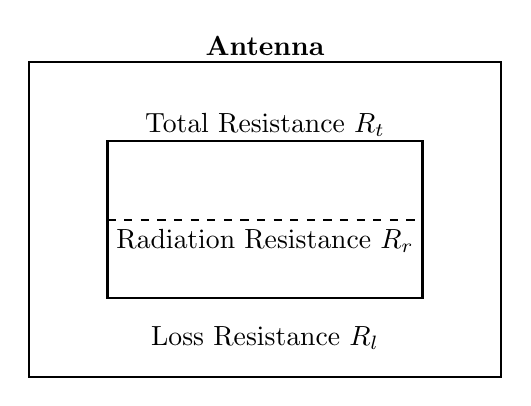
\begin{tikzpicture}
    \draw[thick] (0,0) rectangle (6,4);
    \node at (3,4.2) {\textbf{Antenna}};
    \draw[thick] (1,1) rectangle (5,3);
    \node at (3,3.2) {Total Resistance \(R_t\)};
    \draw[thick, dashed] (1,2) -- (5,2);
    \node[below] at (3,2) {Radiation Resistance \(R_r\)};
    \node at (3,0.5) {Loss Resistance \(R_l\)};
\end{tikzpicture}
\end{center}
